\documentclass[english]{article}
\usepackage{geometry}
\usepackage{hyperref}
\usepackage{inputenc}
\geometry{verbose,tmargin=3.5cm,bmargin=4cm,lmargin=3.8cm,rmargin=3.8cm}
\usepackage[backend=biber,style=ieee]{biblatex}
\addbibresource{sources.bib}
\makeatletter
\usepackage{url}
\usepackage{graphicx}
\usepackage{caption}
\usepackage{wrapfig}
\usepackage{subcaption}
\makeatother
\usepackage{babel}
\usepackage{amsmath}
\usepackage{algorithm}
\newcommand{\Desc}[2]{\State \makebox[2em][l]{#1}#2}
\usepackage[noend]{algpseudocode}
\makeatletter
\def\BState{\State\hskip-\ALG@thistlm}
\makeatother

\begin{document}
	
	\title{Multi-Agent Path Finding with Matching using Increasing Cost Tree Search}
	
	\author{Thom van der Woude\and Jesse Mulderij\and Mathijs de Weerdt}
	\date{}
	
	\maketitle
	
	\begin{abstract}
		Both the assignment problem and the multi-agent pathfinding problem are common problems in fields such as robotics and transportation. The joint problem of finding matchings inducing an optimal non-conflicting routing of agents to their goals is something that has not been studied much. Few methods exist today that solve it although the problems do appear together in real-world problems, such as in the Train Unit Shunting and Servicing problem. In this work, a novel method based on the Increasing Cost Tree Search algorithm for multi-agent pathfinding is presented that can optimally solve this joint problem.
	\end{abstract}
	
	\section{Introduction}
	The Dutch Railways (NS) company\footnote{\url{https://www.ns.nl/}} needs to clean and service their fleet of trains during the night in shunting yards so that they can properly bring passengers from A to B during the day. 
	The problem of scheduling the trains and personnel to achieve this is called the Train Unit Shunting and Servicing (TUSS) problem \cite{mulderij2020}. 
	It is an NP-hard problem with many different subproblems in addition to the basic train unit routing, such as the timetabling of personnel and coupling and decoupling of train units entering and leaving the yard. % introduce heuristics here.
	
	As was shown by Geiger et al.\cite{geiger2018}, in practical scenarios, only heuristic methods can solve TUSS instances. 
	Such methods are suboptimal and heuristic solutions to instances defined for a set shunting yard can be said to characterise a lower bound on the capacity of the shunting yard, as each solution cost gives a (loose) upper bound for the optimal solution cost. 
	The railway company, however, is interested in learning tight upper bounds for the capacity of existing shunting yards to inform decisions about matters like infrastructure expansion. 
	Mulderij et al. \cite{mulderij2020} propose the multi-agent pathfinding (MAPF) problem \cite{stern2019} extended with a matching subproblem (hereafter MAPFM) as a suitable relaxation for finding such upper-bounds using an approach analogous to that outlined above.
	For this to succeed, a way to optimally solve MAPFM instances is needed.
	
	Comparatively, little research has been done on MAPFM and solving MAPFM optimally.
	The Conflict-Based Min-Cost-Flow (CBM) algorithm by Ma and Koenig \cite{ma2016} is one of the few existing approaches to optimally solve this more general problem along with the somewhat similar one described in \cite{henkel2019}.
	Ma and Koenig's method builds upon the conflict-based search method and in particular on the Meta-Agent variation thereof also discussed in \cite{sharon2015} as a high-level search framework, while exploiting the connection between MAPF problems and max-flow problems (as discussed in \cite{yu2013}) in the low-level search. It should be noted that this method minimizes the makespan and not the sum of individual costs which is the objective used in the TUSS relaxation, meaning that non-trivial modifications to CMB are needed to minimize SIC.
	The successful application of CBS to solving MAPFM begs the question: can alternative MAPF algorithms such as Increasing Cost Tree Search (ICTS) \cite{sharon2011} or M* \cite{wagner2011} also serve as the basis for a MAPFM solver?
	
	\begin{wrapfigure}{R}{.25\textwidth}
		\begin{minipage}{\linewidth}
			\centering\captionsetup[subfigure]{justification=centering}
			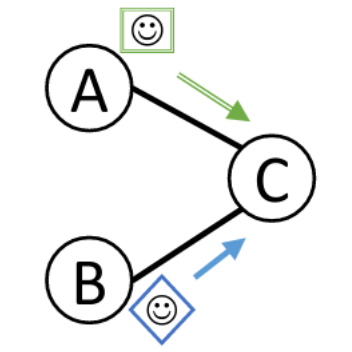
\includegraphics[width=\linewidth]{img/vertex-conflict}
			\subcaption{Vertex conflict}
			\label{fig:conflictsa}\par\vfill
			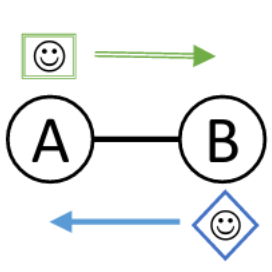
\includegraphics[width=0.75\linewidth]{img/edge-conflict}
			\subcaption{Swapping conflict}
			\label{fig:conflictsb}
		\end{minipage}
		\caption{The two types of conflict (from Fig. 1 in \cite{stern2019})}\label{fig:conflicts}
	\end{wrapfigure}
	This work is the outcome of a search for an efficient algorithm for optimally solving MAPFM derived from ICTS as an alternative to the approach outlined above\footnote{To the knowledge of the author, to date, no such algorithm is described in the literature}. ICTS, in short, is a two-level approach to MAPF with a top-level breadth-first traversal of an Increasing Cost Tree (ICT) representing combinations of per-agent path costs and a bottom-level evaluation of ICT nodes using multi-valued decision diagrams (MDDS). These MDDS represent per agent all possible paths to the goal of a set length. In the context of a research project in which multiple such 
	MAPF algorithms were taken as starting points for MAPFM algorithms within a group, the novel ICTS-based algorithm is compared to these algorithms on a set of benchmarks similar to those described in \cite{stern2019}. In addition, it is analysed in terms of complexity and compared to both an enumerative approach that solves all matchings using regular ICTS and the algorithm described in \cite{ma2016}. Regarding the relevance of this work, it should be noted that besides TUSS, there are other applications such as planning warehouse robots \cite{wurman2007} that also could benefit from novel algorithms for MAPFM.
	
	% Lastly, completeness of the algorithm is considered as this is a key property in the context of MAPFM as a TUSS relaxation.
	\section{Multi-agent pathfinding with matching} % Problem description
	The MAPFM problem is an extension of MAPF, a well-studied problem. Formally, a MAPF instance can be described as follows. Let $G = (V,E)$ be an undirected connected graph, with each $v\in V$ representing an obstacle-free tile on a 4-connected grid and each $e = (u,v)\in E$ representing a legal uniform-cost move between two such tiles. Let there be $k$ agents $a_1,\ldots,a_k$ with respective starting locations $s_1,\ldots,s_k$ and goals $g_1,\ldots,g_k$. For each agent $a_i$, a path $\pi_i$ from $s_i$ to $g_i$ is to be found such that all agents paths $\pi_i$ taken together are non-conflicting and therefore are a solution. In this work, non-conflicting means, in the conflict-terminology of \cite{stern2019}, that there are no vertex conflicts (and thus no edge conflicts) and no swapping conflicts, as shown in Figure \ref{fig:conflicts}. Letting $\pi_i^t$ denote the $t$'th node of path $\pi_i$, this means that for $i\neq j$, for all $t$, $\pi_i^t\neq \pi_j^t$ and $(\pi_i^t \neq \pi_j^{t + 1})\lor(\pi_i^{t+1} \neq \pi_j^t)$. Given a solution $(\pi_1,\ldots,\pi_k)$, a vector of per-agent costs $(c_1,\ldots,c_k)$ can be found. For $\pi_i$, $c_i$ is defined as the time at which $a_i$ reaches $g_i$ for the last time and remains there, meaning that for $t \geq c_i$, $\pi_i^{t} = g_i$. One property of $c_i$ is that $c_i \geq c^*_i$ where $c^*_i$ is defined as the cost of $\pi^*_i$, the shortest path from $s_i$ to $g_i$ that can be computed using any optimal pathfinding algorithm. There are two common objectives in MAPF:
	\begin{itemize}
		\item The makespan: $\max_{i} c_i$
		\item The sum of individual costs (SIC): $\sum_i c_i$
	\end{itemize}
	In this work, following the definition of the TUSS relaxation in \cite{mulderij2020}, an optimal solution is defined as having minimal SIC. Note that $\sum_i c_i \geq \sum_i c^*_i$.
	
	So given a combination of paths $(\pi_1,\ldots,\pi_k)$, a vector of costs is found from which the SIC is derived. This is a surjective mapping: many cost vectors $(c'_1,\ldots,c'_k)$ might add up to the same SIC as $(c_1,\ldots,c_k)$ and for a given agent $a_i$, there might be many equivalent paths $\pi'_i$ to the goal with cost $c_i$. On uniform-cost 4-grids in particular, there are often many equivalent and symmetrical paths\cite{harabor2010} (see Figure \ref{fig:symmetries}), which is why in single-agent pathfinding, symmetry-breaking methods like Jump Point Search\cite{harabor2011} are used to speed up the search. In multi-agent pathfinding, having multiple paths per agent of the same cost can, in contrast, be a boon: it means that there are potentially more non-conflicting ways to combine paths of different agents.
	\subsection{Increasing Cost Tree Search}
	\label{icts}
	\begin{figure}[t]
		\centering
		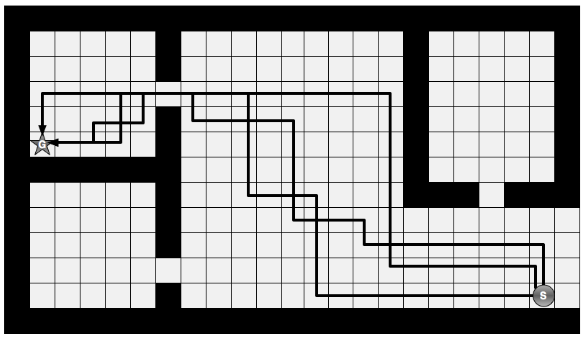
\includegraphics[width=0.4\linewidth]{img/symmetries}
		\caption{Symmetric paths on a 4-connected grid\cite{harabor2010}}
		\label{fig:symmetries}
	\end{figure}
	In Increasing Cost Tree Search\cite{sharon2011}, the above two-step mapping from path combination to SIC is reversed to search for a solution with minimal SIC. This is done by searching for cost vectors corresponding to increasing SIC on the top level and searching for non-conflicting path combinations (solutions) for each cost vector on the bottom level. 
	
	\subsubsection{Top-level search}
	In the top-level search, all possible cost vectors for a given SIC are evaluated by searching an Increasing Cost Tree as depicted in \ref{fig:ict}, starting from $C_{root} = \sum_i c^*_i$ corresponding to a single root cost vector $(c^*_1,c^*_2,\ldots,c^*_k)$. This root has $k$ children $(c^*_1 + 1,c^*_2,\ldots,c^*_k),(c^*_1,c^*_2 + 1,\ldots,c^*_k),\ldots,(c^*_1,c^*_2,\ldots,c^*_k + 1)$ all of cost $C = C_{root} + 1$. Searching this ICT breadth-first corresponds to evaluating all possible cost vectors corresponding to increasing cost $C$ starting with $C_{root}$, guaranteeing optimality of a found solution. The number of cost vectors evaluated when searching up to nodes of cost $C_{root} + \Delta$ is $\mathcal{O}(k^\Delta)$. Node evaluation is done by a low-level search that searches for a solution $(\pi_1,\ldots,\pi_k)$ corresponding to the node costs $(c_1,\ldots,c_k)$.
	
	\begin{figure}[t]
		\centering
		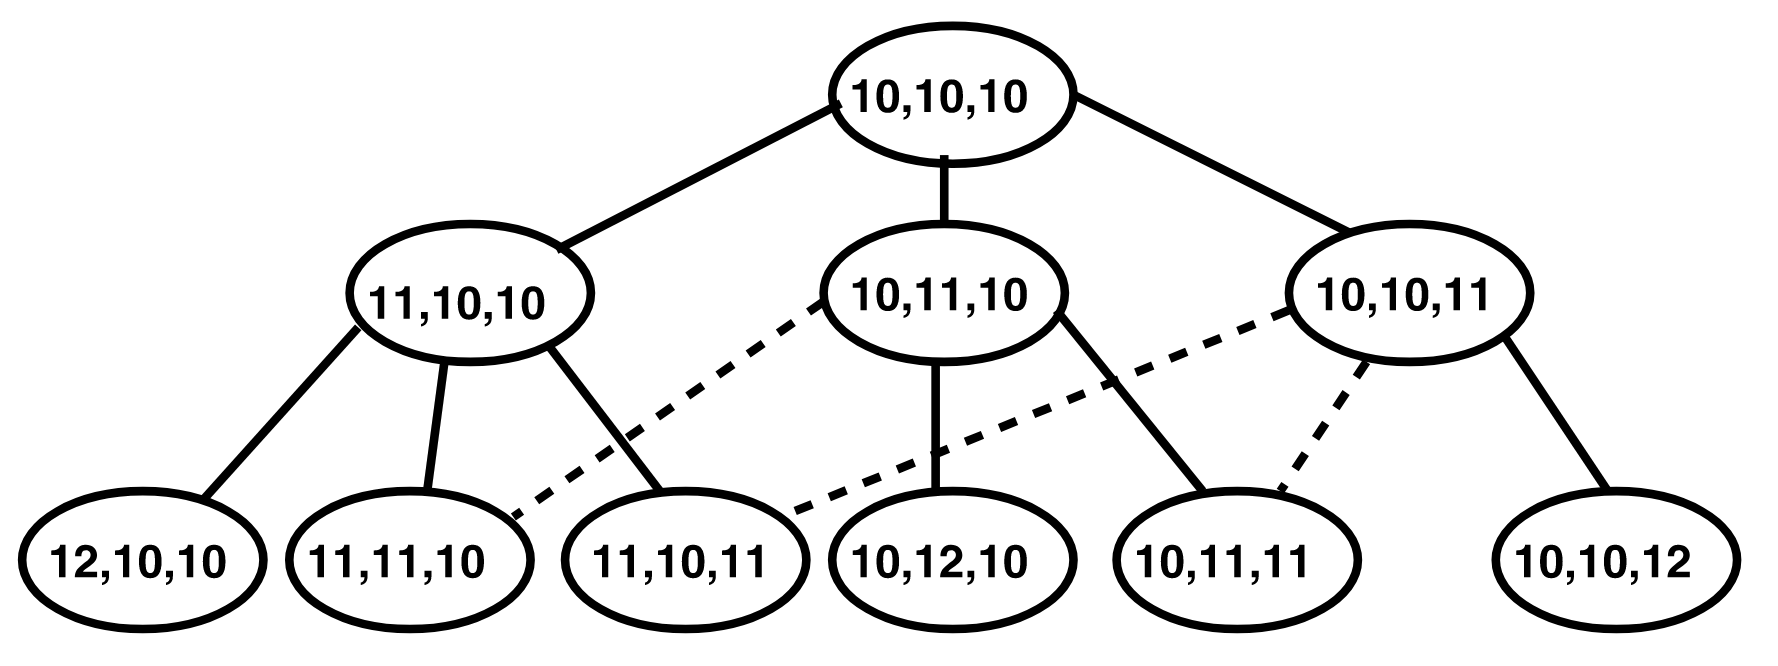
\includegraphics[width=0.7\linewidth]{img/ict}
		\caption{Increasing Cost Tree for three agents \cite{sharon2011}}
		\label{fig:ict}
	\end{figure}
	\begin{figure}
		
	\end{figure}
	
	
	\begin{figure}[b]
		\centering
		\begin{subfigure}{0.2\textwidth}
			\centering
			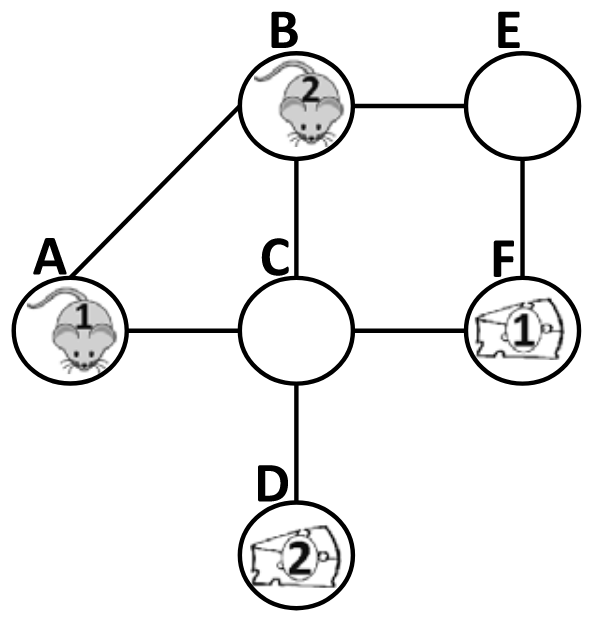
\includegraphics[width=\linewidth]{img/mdds1}
			\caption{An example problem}
			\label{fig:problem}
		\end{subfigure}
		\hfill
		\begin{subfigure}{0.3\textwidth}
			\centering
			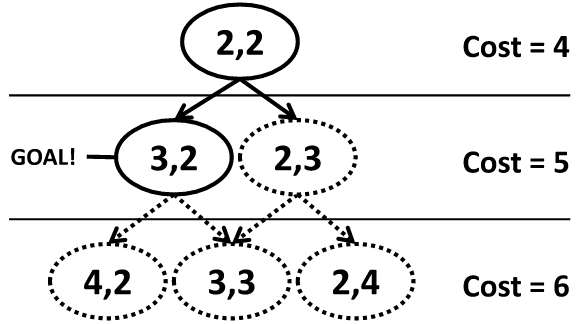
\includegraphics[width=\linewidth]{img/ict2}
			\caption{The corresponding ICT with solution node $(3,2)$}
			\label{fig:ict2}
		\end{subfigure}
		\hfill
		\begin{subfigure}{0.4\textwidth}
			\centering
			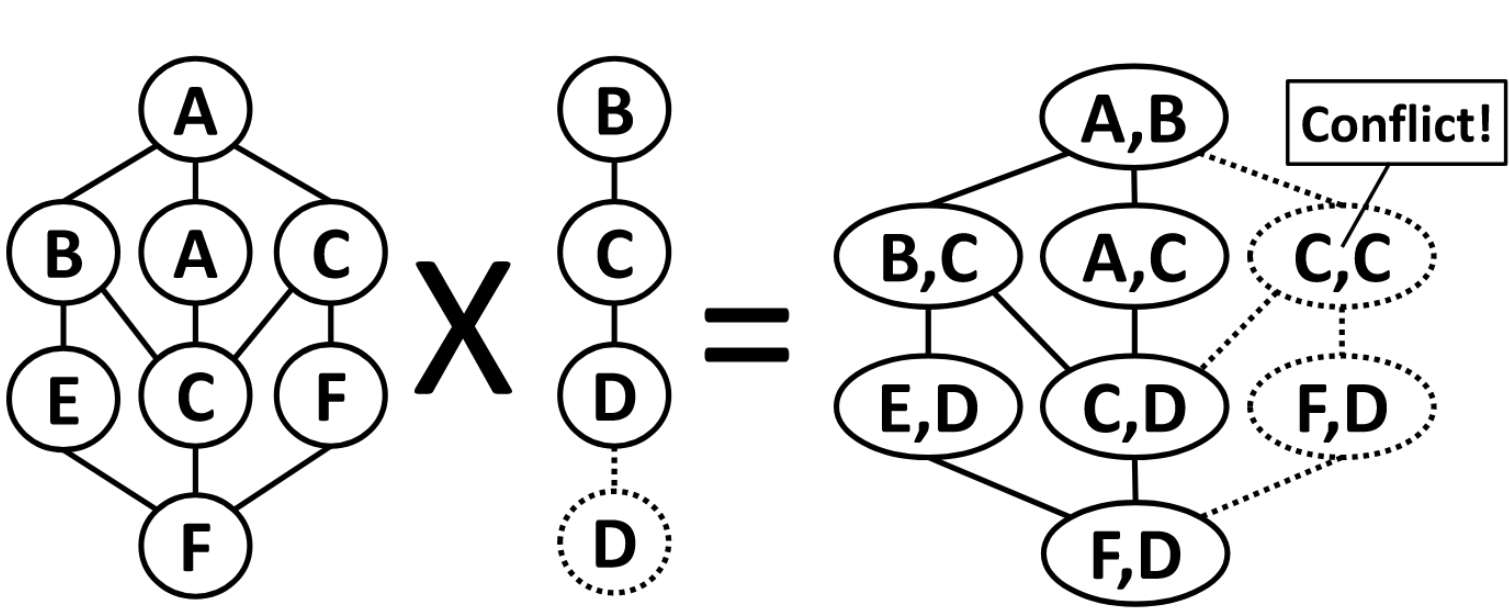
\includegraphics[width=\linewidth]{img/mdds}
			\caption{MDDs for the agents are found and combined}
			\label{fig:mdds}
		\end{subfigure}
		
		\caption{Example of using ICTS to solve MAPF from \cite{sharon2011}}
		\label{fig:bottom}
	\end{figure}
	\subsubsection{Bottom-level search}
	Explicitly generating all paths to the goal for agent $a_i$ of cost $c_i$ is expensive: the number of paths is exponential in $c_i$. This is why in the low-level search of ICTS, multi-valued decision diagrams (MDDs) are used to compactly represent all paths per agent. For $a_i$ with a target cost $c_i$ (from cost vector), $MDD_i^{c_i}$ can be generated by a breadth-first search on the $c_i$-steps time-expanded graph starting at $s_i$, followed by a process similar to the standard path reconstruction method used in A* but allowing multiple node parents. Storing the resulting paths in an MDD, which has at most $|V|$ nodes at each timestep or depth, avoids the cost of storing all paths explicitly and facilitates the efficient search of the $k$-agent space of path combinations.
	
	In Figure \ref{fig:bottom}, a problem with its corresponding ICT is shown, as well as the low-level search of the (solution) node $(3,2)$ using MDDs. Note that the second agent staying at node D after completing the path is modelled in its MDD also to ensure that the place remains blocked.
	
	Subfigure \ref{fig:mdds} illustrates how two or more MDDs can be combined: first, the root nodes are joined; next, the product of the children of both roots is taken and checked for conflicts. In \ref{fig:mdds}, a vertex conflict occurs and therefore this joint child can be removed from the MDD. If a $(B,A)$ node would be generated by the same root, $(A,B)$, this would similarly be a swapping conflict and hence $(B,A)$ would also be removed from the joint MDD $MDD_{1,2}^{c_1,c_2}$. In the next layer, the process repeats with multiple parent nodes.
	
	In practice, joint MDDs are not explicitly constructed but instead, a depth-first search is used to search joint MDDs. This has the benefit of finding a path to the bottom of the joint MDD fast if one exists, while not constructing more of the joint MDD (which can get rather large) than is necessary for finding a solution.
	\subsubsection{ICTS with Independence Detection}
	Like many other MAPF algorithms, ICTS can be embedded in the Independence Detection (ID) framework introduced by Standley in \cite{standley2010}. ID starts by assuming each agent is a group that can be assigned an optimal path independent of other groups. If group paths do conflict, they become one group that is planned together using a MAPF algorithm, in this case, ICTS, until no conflicts between groups occur. The goal of ID is to minimize $k'$, the size of the largest group that has to be planned. Optionally, a conflict avoidance table (CAT) can be maintained for use during the planning of groups. This records the paths planned by other groups and can facilitate tie-breaking in search that minimizes the number of conflicts; the CAT is omitted from Algorithm \ref{id-algo} for brevity but was implemented and used in experiments.
	\begin{algorithm}
		\begin{algorithmic}[1]
			\State \text{Assign each agent to a singleton group}
			\State \text{plan a path for each group}
			\Repeat
			\State \text{simulate execution of all paths until a conflict occurs}
			\State \text{merge two conflicting groups into a single group}
			\State \text{cooperatively plan new group}
			\Until{\text{no conflicts occur}}
			\State $solution\gets\text{paths of all groups combined}$
			\State \textbf{return solution}
		\end{algorithmic}
		\caption{Simple Independence Detection by Standley} 
		\label{id-algo}
	\end{algorithm}
	
	\subsubsection{Pruning in ICTS}
	\label{pruning}
	In \cite{sharon2011}, in addition to the basic two-level solver, three pruning methods to speed up search are discussed, two of which were used in this work. All work by taking $j < k$ and applying the described method to each possible combination of $j$ out of $k$ agents. If no solution exists for any such combination, the full $k$-agent low-level search is not triggered. The two basic pruning methods are as follows.
	\begin{enumerate}
		\item Simple pruning: the $j$-agent MDD is searched using DFS for a solution.
		\item Enhanced pruning: the $j$-agent MDD is searched using BFS and when children are generated, for each agent, all children that do not appear in any unified node are removed from the MDD. In \ref{fig:mdds}, the $C$ node of $MDD_1$ would be removed as it cannot be unified with any node of $MDD_2$ at that level. 
	\end{enumerate}
	In addition, repeated enhanced pairwise pruning is described in which the enhanced pruning procedure is repeated for all combinations until a fixpoint is reached, which is when no child node is removed from any of the agent MDDs in an iteration. This was not used in this work. 
	
	The full ICT-search algorithm including a pruning step is described by Algorithm \ref{icts-algo}. It is reproduced from \cite{sharon2011} for completeness. As noted before, this procedure could be used for planning groups in Algorithm \ref{id-algo}. 
	\begin{algorithm}
		\begin{algorithmic}[1]
			\Procedure{ICT-search}{MAPF instance}
			\State \text{Construct ICT root}
			\ForAll{\text{ICT nodes }$(c_1,\ldots,c_k)$\text{ in breadth-first order }} 
			\ForAll{\text{agents} $a_i$} 
			\text{Construct} $MDD_i^{c_i}$
			\EndFor
			\ForAll{$j$-\text{agent combinations} $(i_1,\ldots,i_j)$} 
			\State \text{Run node-pruning procedure with MDDs }$MDD_{i_1}^{c_{i_1}},\ldots,MDD_{i_j}^{c_{i_j}}$
			\If{\text{no solution was found for a combination in pruning}}
			\State \textbf{Break}\text{ and continue with next ICT node}
			\EndIf
			\EndFor
			\State \text{Search }$k$\text{-agent MDD space}
			\If{\text{solution was found}}
			\State \textbf{return solution}
			\EndIf
			\EndFor
			
			\EndProcedure
		\end{algorithmic}
		\caption{Increasing Cost Tree Search}
		\label{icts-algo}
	\end{algorithm}
	\subsection{Extending MAPF with matching}
	With the multi-agent pathfinding problem as well as the ICTS method of solving it defined, the matching extension of MAPF (MAPFM) that is the subject of this paper can be described. Possible extensions of ICTS to match these changes will be discussed in Section \ref{section:icts-matching}.
	
	Let there be $K$ teams $t_1,\ldots, t_K$, where $t_i$ consists of $k_i$ agents with start positions $s_1^i,\ldots,s_{k_i}^i$ together with an equal number of team goals $g_1^i,\ldots,g_{k_i}^i$. Within each team $t_i$, agent $a_j^i$ are to be \textit{matched} to a unique goal $g_k^i$, so that exactly one agent is assigned to each goal within team $i$; once all agents are matched to goals, for each agent $a_j^i$ matched to $g_k^i$, a path from $s_j^i$ to $g_k^i$ is to be found such that all agents paths taken together are non-conflicting and therefore make up a solution \cite{ma2016}, similarly defined as for MAPF.
	
	
	%
	\section{Solving MAPF with Matching using ICTS} % Your contribution
	\label{section:icts-matching}
	Taking ICTS for MAPF as starting point, two methods to use ICTS for MAPFM were identified. The first method relies on the well-known reduction from MAPFM to repeated MAPF: an optimal solution to MAPFM corresponds to a matching of agents to goals, so by exhaustively enumerating all matchings and solving these as MAPF instances, an optimal solution to the MAPFM instance can be found. In the second method, the increasing cost trees search itself is modified to allow an agent $a_j^i$ to be matched to any $g_k^i$. For each method, some properties and method-specific optimizations and variations will be discussed. Afterwards, some more general considerations will be discussed.
	\subsection{Exhaustive ICTS}
	For $K$ teams $t_1,\ldots,t_K$ of size $k_i$, there are in total $M = \prod_{i} k_i!$ matchings from team agents to team goals. Let $C_1$ through $C_M$ denote the optimal SIC costs of each MAPF instance corresponding to the instance, with $C_m = \infty$ for unfeasible $m$. Let $\Delta_m$ be similarly defined and represent the difference between $C_m$ and the root cost of $m$. In order to find the optimal solution, $m$ with lowest $C_m$ has to be found, which requires all $M$ to be solved or marked as unfeasible, meaning that $\mathcal{O}(M)$ MAPF instances have to be solved. 
	
	However, once the first solution is found with cost $C_m$, this can be used in the next search as an (exclusive) upper-bound $B$ for the SIC of nodes. Formally, let $B = \infty$ represent the initial SIC bound of the ICT search. After solving each $C_m$, let $B_{m+1} = \min(B_m,C_m)$. By successively updating this $B$ in this manner, as more matchings are solved, the effort needed to solve the remaining matchings can be expected to be reduced significantly.
	
	As a further improvement of this method, the order in which matchings are enumerated and solved could be changed. In particular, by sorting the matchings in increasing order of root SIC, it can be seen that $\Delta'_{m + 1}$, the distance from $B_{m+1}$ or the solution to matching $m + 1$ (whichever was reached first) and the root SIC, will always be less or equal to the $\Delta'_m$ [TODO: proof]. Although this is itself a promising property, to make use of it, all roots have to be computed and all $M$ corresponding SIC values have to be sorted which is a $\mathcal{O}(M\log M)$ procedure. 
	
	\subsection{ICTS-m}
	ICTS with Matching (ICTS-m) generalizes ICTS to optimally solve MAPFM instances. Few changes to ICTS were necessary to accommodate for matching in this increasing cost tree scheme. Specifically, the ICT root generation and the MDD generation had to be changed. As described in \ref{icts}, in ICTS the root cost for each agent $a_i$ is given by $c^*_i$, the cost of the shortest path from $s_i$ to $g_i$, i.e. without taking conflicts into account. $MDD_i^{c_i}$ is generated using a breadth-first search from $s_i$ to $g_i$ followed by some additional processing.
	\subsubsection{Root generation for matching}
	Given a team $t_i$ of size $k_i$, for any agent $a_j^i$ there are $k_i$ costs $c_j(1),c_j(2),\ldots,c_j(k_i)$ for shortest paths from $s_j^i$ to each goal $g_k^i$. Making no assumptions about what goals other agents in $t_i$ are assigned to, it could be that in the optimal solution $a_j^i$ is assigned to a goal $g_{m}^i$ with path cost $c^*_j = c_j(m)$ such that $c_j(m) = \min_{n\in\{0,\ldots,k_i\}} c_j(n)$. Therefore, to guarantee optimality, this minimal cost to any matching goal has to take the place of the shortest path cost from the original ICTS root. The resulting root is equivalent to that generated in regular ICTS in the case that all teams are singleton, which is equivalent to a MAPF instance. Intuitively, the sum of individual costs of this root is highly optimistic, in particular, if the teams are large. This is because often, agents will not move to their closest matching goal in an optimal solution, even without considering conflicts.
	
	\subsubsection{MDD generation for matching}
	In MDD generation, each agent also has to consider not one goal but all matching goals. By following a BFS-based approach, with all team goals being goals in the search and in turn endpoints from which, using the time-expanded graph, the MDD was generated that is used in the low-level search, agent MDDs can be made to represent all possible paths of a set length to any matching goal. Once again, if all teams are singleton, the MDDs generated using this goal-set approach are the same as in regular ICTS.
	\begin{wrapfigure}{R}{.35\textwidth}
		\centering
		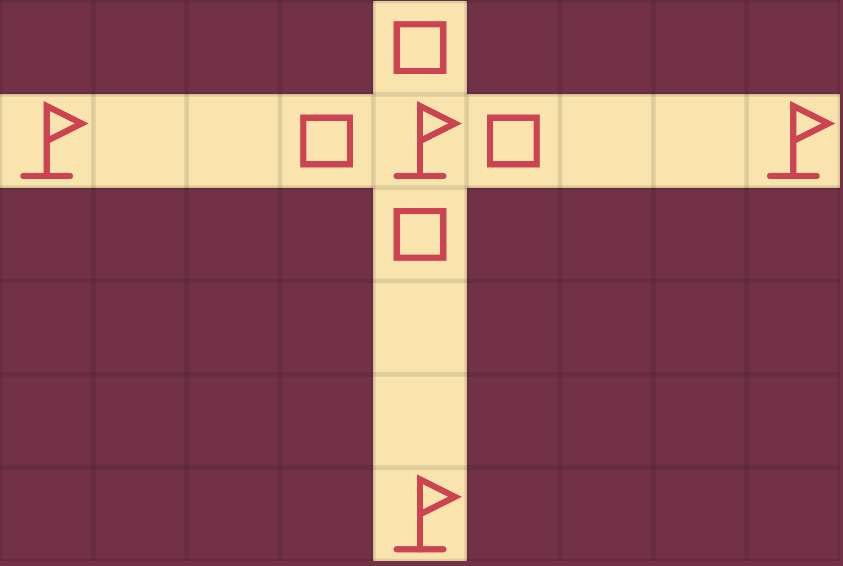
\includegraphics[width=\linewidth]{img/path}
		\caption{Pathelogical case for ICTS-m [Placeholder graphic]}
		\label{fig:path}
	\end{wrapfigure}
	\subsubsection{Properties of ICTS-m}
	As a consequence of the $\min$ operation in the root definition, a pathological case can be derived. Consider a team of 4 agents $a_1^1$ through $a_4^1$. Let them be arranged in a configuration as depicted in Figure \ref{fig:path}. As indicated by the color, all four agents match the colour of the centre goal and hence for each $i$, $c^*_i = 1$, so that the root is $(1,1,1,1)$ with SIC $4$. The optimal solution however is, numbering the agents clockwise, $(1,3,3,3)$ with SIC $10$, meaning that $\Delta = 6$. It can be seen that instances of this form with arbitrarily large $\Delta$ can be constructed. As ICTS-m being a generalization of ICTS is $\mathcal{O}(k^\Delta)$, even just extending the 'limbs' of the instance to yield an ICT root of $(1,9,9,9)$ with $\Delta = 24$ will result in an unfathomably large number of nodes being evaluated assuming no pruning or other modifications to the base algorithm.
	\subsection{General optimization: child pruning}
	An optimization of ICTS that hitherto appears to not have been described in the literature was found in the process of optimizing ICTS-m. The idea is simple: when pruning, in the original ICTS formulation all $k$-children are generated in every case because pruning only controls skipping the low-level search, assumed to be the most expensive operation. However, in simple pruning in any case, when there is a conflict between two or more agents at a given ICT node $(c_1,\ldots,c_k)$, in any solution, one or more of the path costs corresponding to these conflicting agents will have to be incremented in any solution node. This reduces the number of children generated to the number of conflicting agents, which quite drastically can improve the branching factor of the ICT search if say $k = 12$ but a conflicting pair is found.
	
	It is conjectured that child pruning combined with enhanced pruning does not in general guarantee optimality, but despite extensive search no counter-example has been found. [TODO: find counter-example/proof optimality]
	\begin{figure*}
		\centering
		\begin{subfigure}{0.49\textwidth}
			\centering
			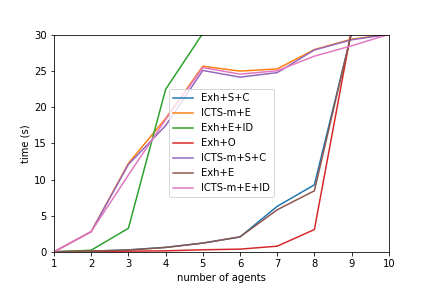
\includegraphics[width=\linewidth]{img/results/open-1}
			\caption{Open, 1 team}
			\label{fig:open1}
		\end{subfigure}
		\begin{subfigure}{0.49\textwidth}
			\centering
			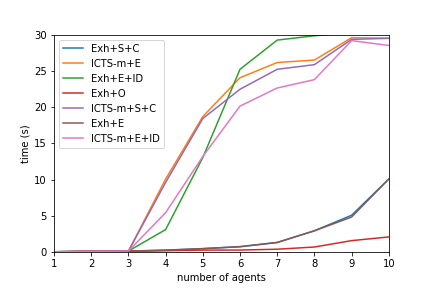
\includegraphics[width=\linewidth]{img/results/open-3}
			\caption{Open, 3 teams}
			\label{fig:open3}
		\end{subfigure}
		\begin{subfigure}{0.49\textwidth}
			\centering
			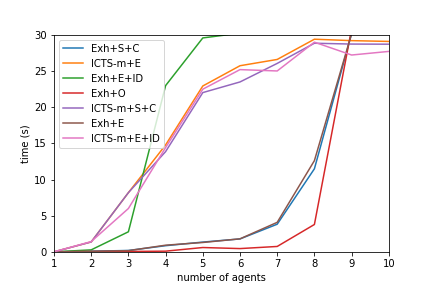
\includegraphics[width=\linewidth]{img/results/obstacle-1}
			\caption{Obstacle, 1 team}
			\label{fig:obstacle1}
		\end{subfigure}
		\begin{subfigure}{0.49\textwidth}
			\centering
			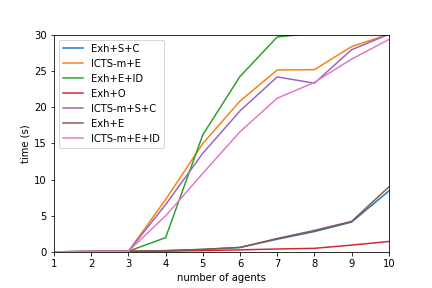
\includegraphics[width=\linewidth]{img/results/obstacle-3}
			\caption{Obstacle, 3 teams}
			\label{fig:obstacle3}
		\end{subfigure}
		\begin{subfigure}{0.49\textwidth}
			\centering
			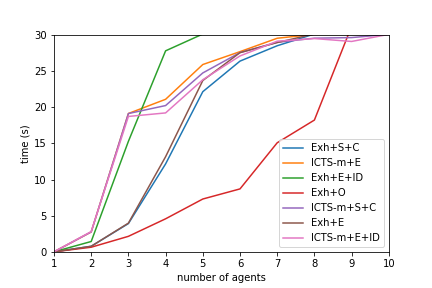
\includegraphics[width=\linewidth]{img/results/maze-1}
			\caption{Maze, 1 team}
			\label{fig:m1}
		\end{subfigure}
		\begin{subfigure}{0.49\textwidth}
			\centering
			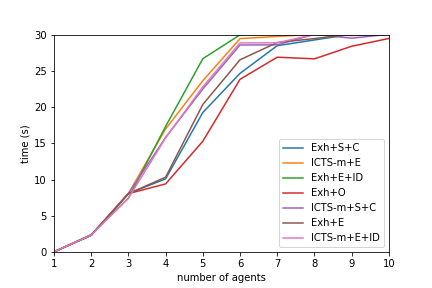
\includegraphics[width=\linewidth]{img/results/maze-3}
			\caption{Maze, 3 teams}
			\label{fig:m3}
		\end{subfigure}
		\caption{Average solving time of algorithm variants on various types of 20x20 grids with a 30s timeout}
		\label{fig:times}
	\end{figure*}
	
	\begin{figure*}
		\centering
		\begin{subfigure}{0.49\textwidth}
			\centering
			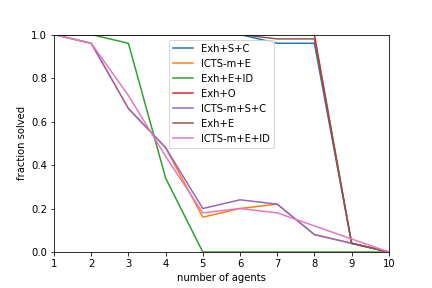
\includegraphics[width=\linewidth]{img/results/open-1-p}
			\caption{Open, 1 team}
			\label{fig:open1p}
		\end{subfigure}
		\begin{subfigure}{0.49\textwidth}
			\centering
			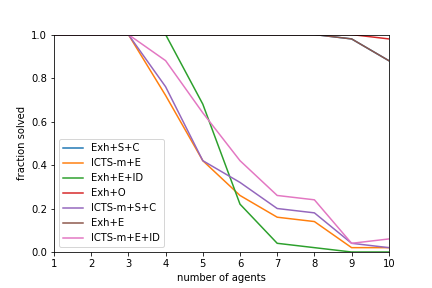
\includegraphics[width=\linewidth]{img/results/open-3-p}
			\caption{Open, 3 teams}
			\label{fig:open3p}
		\end{subfigure}
		\begin{subfigure}{0.49\textwidth}
			\centering
			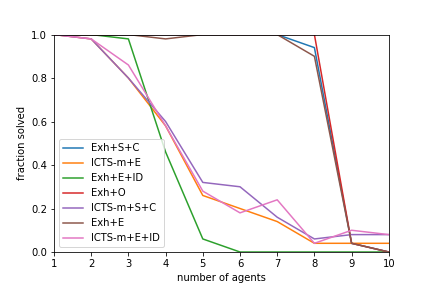
\includegraphics[width=\linewidth]{img/results/obstacle-1-p}
			\caption{Obstacle, 1 team}
			\label{fig:obstacle1p}
		\end{subfigure}
		\begin{subfigure}{0.49\textwidth}
			\centering
			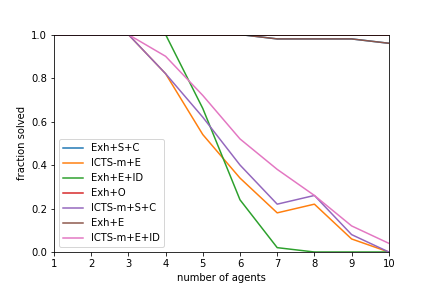
\includegraphics[width=\linewidth]{img/results/obstacle-3-p}
			\caption{Obstacle, 3 teams}
			\label{fig:obstacle3p}
		\end{subfigure}
		\begin{subfigure}{0.49\textwidth}
			\centering
			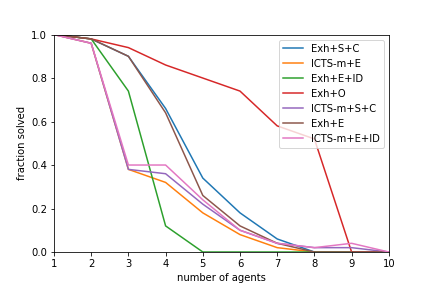
\includegraphics[width=\linewidth]{img/results/maze-1-p}
			\caption{Maze, 1 team}
			\label{fig:maze1p}
		\end{subfigure}
		\begin{subfigure}{0.49\textwidth}
			\centering
			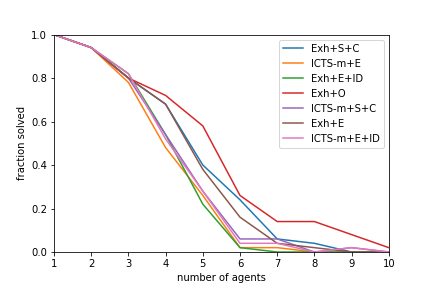
\includegraphics[width=\linewidth]{img/results/maze-3-p}
			\caption{Maze, 3 teams}
			\label{fig:maze3p}
		\end{subfigure}
		\caption{Fraction solved out of 50 maps of algorithm variants on various types of 20x20 grids with a 30s timeout}
		\label{fig:probs}
	\end{figure*}
	
	\section{Experiments}
	Because MAPFM lies on the fringe of pathfinding research, no standard benchmarks exist\footnote{That is, to the knowledge of the author.}. For MAPF, there are the Moving AI benchmarks \cite{sturtevant2012} and potentially a new MAPFM standard benchmark could be defined by generating suitable partitions of agents into teams for these MAPF instances. It was noticed however that optimally solving even small MAPFM instances with comparatively few agents and short distances to goals was computationally already a challenge. This observation informed the creation of a map generator within the peer group with various parameters. Using this map generator, three types of 20x20 grids were generated:
	\begin{enumerate}
		\item Open: An obstacle-free grid
		\item Obstacle: A grid with some obstacles
		\item Maze: A grid with many obstructed tiles
	\end{enumerate}
	For each of these types, two sets of maps were generated with between $1$ and $10$ agents and 50 instances generated for each such agent-setting: one set where all agents belong to one team, another in which the agents were divided into three teams (or $1,2$ teams respectively for the datapoints with $1,2$ agents). The results are shown in Figure \ref{fig:times} and \ref{fig:probs}, which respectively show the average time to solution and the fraction of problems solved out of 50 instances. The algorithms and interpretation of results are discussed below.
	\subsection{Algorithms}
	Various improvements and variations of algorithms were tried out, as shown in the legend. S and E denote simple and enhanced pruning respectively; ID means that Independence Detection was used; C means that child pruning was used.
	\subsection{Results}
	A first observation is that exhaustive methods, while dominant throughout all settings, fare much better when agents are divided into three teams as opposed to when there is just one team. This can be explained by exhaustive algorithms having to process $M = k!$ matchings, which grows quite large for say $k = 10$. Another is that simple pruning combined with child pruning appears to outperform enhanced in many cases, as in Subfigure \ref{fig:maze1p}. More analysis is necessary however before any conclusions can be drawn.
	
	
	\section{Responsible Research}
	In experiments used to compare the different MAPFM algorithms within the peer group, care was taken to make the comparison fair: all algorithms are implemented in Python 3 and run on the same system: a server with a 12-core Intel Xeon E5-2683 with 8Gb of RAM dedicated to running experiments for this project. Still, some implementations might be more optimized than others so this might be a factor in performance characteristics and in particular in relative performance differences.
	
	The implementation of the ICTS-based algorithms described in this work is publicly available online in the form of a Github repository \footnote{\url{https://github.com/tbvanderwoude/icts-m}}. Included is also code used to benchmark different configurations of the ICTS solver.
	
	\section{Discussion}
	Compared to the results achieved by \cite{ma2016}, the results recorded are somewhat disappointing.
	\section{Conclusions}
	The goal of this research was to seek alternative approaches to solving MAPFM based on ICTS. In this, the research has succeeded, but the performance and in particular the scalability of the algorithms leaves something to be desired. 
	\section{Future work}
	The ICTS-m algorithm described in this work scales quite poorly for several reasons including the highly optimistic root SIC value. It might be possible to conceive of a different ICTS-m algorithm that is better able to take advantage of the agents being divided into teams, for instance by first solving all intra-team conflicts before proceeding to consider inter-team conflicts. Some early experiments with pruning techniques were in this vein but experimentally there was no observable improvement.
	\printbibliography
	
\end{document}
